% Options for packages loaded elsewhere
\PassOptionsToPackage{unicode}{hyperref}
\PassOptionsToPackage{hyphens}{url}
%
\documentclass[
  12pt,
]{book}
\usepackage{lmodern}
\usepackage{setspace}
\usepackage{amsmath}
\usepackage{ifxetex,ifluatex}
\ifnum 0\ifxetex 1\fi\ifluatex 1\fi=0 % if pdftex
  \usepackage[T1]{fontenc}
  \usepackage[utf8]{inputenc}
  \usepackage{textcomp} % provide euro and other symbols
  \usepackage{amssymb}
\else % if luatex or xetex
  \usepackage{unicode-math}
  \defaultfontfeatures{Scale=MatchLowercase}
  \defaultfontfeatures[\rmfamily]{Ligatures=TeX,Scale=1}
\fi
% Use upquote if available, for straight quotes in verbatim environments
\IfFileExists{upquote.sty}{\usepackage{upquote}}{}
\IfFileExists{microtype.sty}{% use microtype if available
  \usepackage[]{microtype}
  \UseMicrotypeSet[protrusion]{basicmath} % disable protrusion for tt fonts
}{}
\makeatletter
\@ifundefined{KOMAClassName}{% if non-KOMA class
  \IfFileExists{parskip.sty}{%
    \usepackage{parskip}
  }{% else
    \setlength{\parindent}{0pt}
    \setlength{\parskip}{6pt plus 2pt minus 1pt}}
}{% if KOMA class
  \KOMAoptions{parskip=half}}
\makeatother
\usepackage{xcolor}
\IfFileExists{xurl.sty}{\usepackage{xurl}}{} % add URL line breaks if available
\IfFileExists{bookmark.sty}{\usepackage{bookmark}}{\usepackage{hyperref}}
\hypersetup{
  pdftitle={Estudio Longitudinal Social de Chile},
  hidelinks,
  pdfcreator={LaTeX via pandoc}}
\urlstyle{same} % disable monospaced font for URLs
\usepackage[left=4cm, right=3cm, top=2.5cm, bottom=2.5cm]{geometry}
\usepackage{longtable,booktabs}
% Correct order of tables after \paragraph or \subparagraph
\usepackage{etoolbox}
\makeatletter
\patchcmd\longtable{\par}{\if@noskipsec\mbox{}\fi\par}{}{}
\makeatother
% Allow footnotes in longtable head/foot
\IfFileExists{footnotehyper.sty}{\usepackage{footnotehyper}}{\usepackage{footnote}}
\makesavenoteenv{longtable}
\usepackage{graphicx}
\makeatletter
\def\maxwidth{\ifdim\Gin@nat@width>\linewidth\linewidth\else\Gin@nat@width\fi}
\def\maxheight{\ifdim\Gin@nat@height>\textheight\textheight\else\Gin@nat@height\fi}
\makeatother
% Scale images if necessary, so that they will not overflow the page
% margins by default, and it is still possible to overwrite the defaults
% using explicit options in \includegraphics[width, height, ...]{}
\setkeys{Gin}{width=\maxwidth,height=\maxheight,keepaspectratio}
% Set default figure placement to htbp
\makeatletter
\def\fps@figure{htbp}
\makeatother
\setlength{\emergencystretch}{3em} % prevent overfull lines
\providecommand{\tightlist}{%
  \setlength{\itemsep}{0pt}\setlength{\parskip}{0pt}}
\setcounter{secnumdepth}{5}
\usepackage[utf8]{inputenc}
\usepackage[spanish]{babel}
\usepackage{geometry}
\geometry{letterpaper,left=2cm,top=2cm, right=2cm}
\usepackage{times}           
\usepackage{caption}
\captionsetup[figure, table]{labelfont={bf},labelformat={default},labelsep=period}
\usepackage{graphicx}
\usepackage{float}
\usepackage{booktabs}
\usepackage{longtable}
\usepackage{array}
\usepackage{multirow}
\usepackage{wrapfig}
\usepackage{float}
\usepackage{colortbl}
\usepackage{xcolor}
\usepackage{pdflscape}
\usepackage{tabu}
\usepackage{threeparttable}
\usepackage{pdfpages} %para pdf portada
\usepackage{fancyhdr} %headers

% fuente: https://stackoverflow.com/questions/45963505/coverpage-and-copyright-notice-before-title-in-r-bookdown
\let\oldmaketitle\maketitle 
\AtBeginDocument{\let\maketitle\relax}




\pagestyle{fancy}
\fancyhf{}
\fancyhead[R]{\emph{\nouppercase{\rightmark}}}
\fancyhead[L]{\emph{\nouppercase{\thepage}}}
% \fancyfoot[CE,CO]{\leftmark}
% \fancyfoot[LE,RO]{\thepage}

\renewcommand{\headrulewidth}{1pt}
% \renewcommand{\footrulewidth}{1pt}

\usepackage{booktabs}
\usepackage{longtable}
\usepackage{array}
\usepackage{multirow}
\usepackage{wrapfig}
\usepackage{float}
\usepackage{colortbl}
\usepackage{pdflscape}
\usepackage{tabu}
\usepackage{threeparttable}
\usepackage{threeparttablex}
\usepackage[normalem]{ulem}
\usepackage{makecell}
\usepackage{xcolor}
\ifluatex
  \usepackage{selnolig}  % disable illegal ligatures
\fi
\usepackage[]{natbib}
\bibliographystyle{apalike}

\title{Estudio Longitudinal Social de Chile}
\usepackage{etoolbox}
\makeatletter
\providecommand{\subtitle}[1]{% add subtitle to \maketitle
  \apptocmd{\@title}{\par {\large #1 \par}}{}{}
}
\makeatother
\subtitle{Resultados longitudinales 2016-2019}
\author{}
\date{\vspace{-2.5em}2020-12-24}

\begin{document}
\maketitle

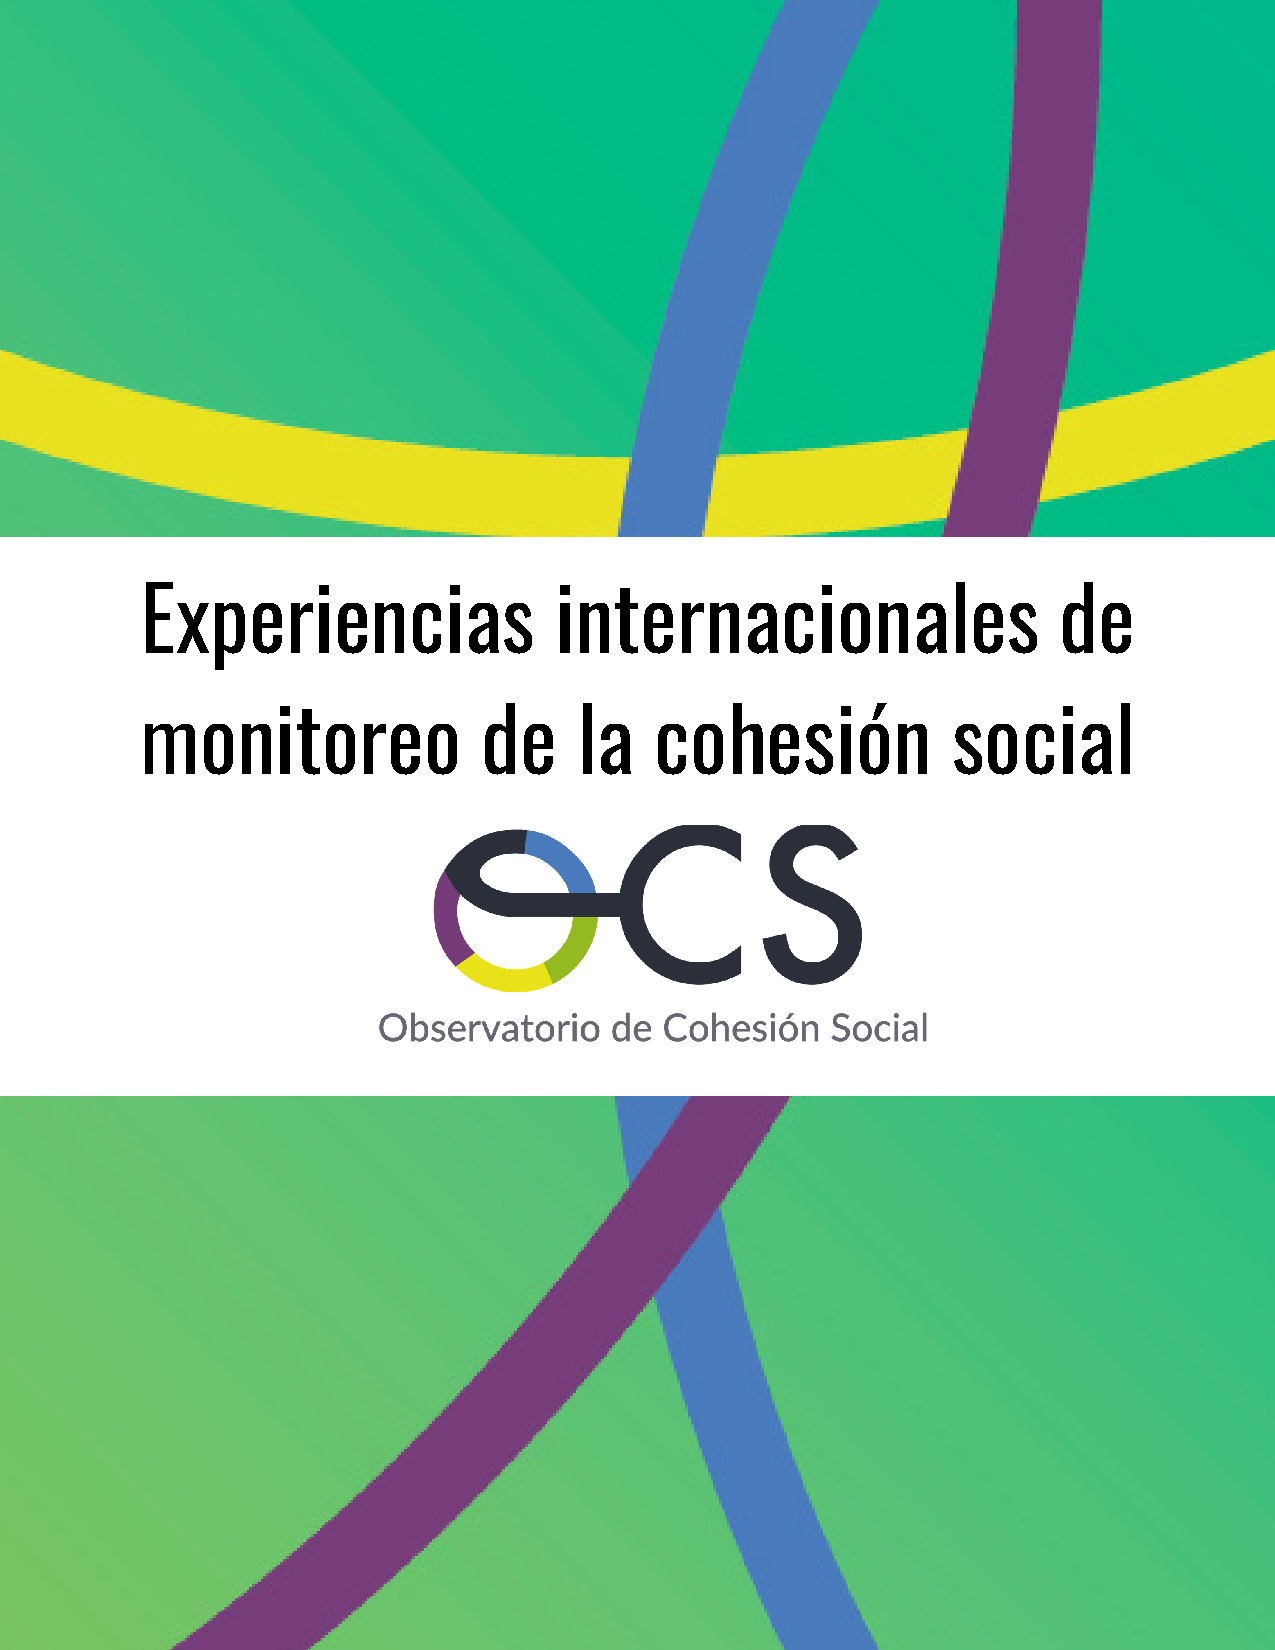
\includepdf[pages={1},scale=1.0]{inputs/frontpage.pdf}	

{
\setcounter{tocdepth}{1}
\tableofcontents
}
\listoftables
\listoffigures
\setstretch{1.5}
\hypertarget{introducciuxf3n-al-reporte}{%
\chapter{Introducción al reporte}\label{introducciuxf3n-al-reporte}}

\begin{center}
\includegraphics[width=0.7\linewidth]{inputs/images/logos} \end{center}

El Centro de Estudios de Conflicto y Cohesión Social (COES) desarrolla investigación colaborativa en temas relacionados al conflicto social y la cohesión (convivencia) en Chile, por medio de un equipo multidisciplinario proveniente de las ciencias sociales y humanidades. COES centra sus actividades académicas y de difusión en el análisis de las múltiples manifestaciones del conflicto y cohesión social en Chile, sus causas, así como también su contexto cultural e histórico.

COES está patrocinado por la Universidad de Chile y la Pontificia Universidad Católica de Chile, y como instituciones asociadas se encuentran la Universidad Diego Portales y la Universidad Adolfo Ibáñez. COES cuenta con el apoyo del Fondo de Financiamiento de Centros de Investigación en Áreas Prioritarias (FONDAP, dependiente de la Agencia Nacional de Investigación y Desarrollo (ANID) del Ministerio de Ciencia, Tecnología, Conocimiento e Innovación. ELSOC además cuenta como socio al Instituto Milenio para la Investigación en Depresión y Personalidad (MIDAP).

\begin{center}
\includegraphics[width=0.3\linewidth]{inputs/images/anid_midap} \end{center}

\hypertarget{equipo-ejecutivo}{%
\section{Equipo Ejecutivo}\label{equipo-ejecutivo}}

\textbf{Roberto González}

Profesor Titular Escuela de Psicología PUC. Investigador Principal COES

\textbf{Matías Bargsted}

Profesor Asociado Instituto de Sociología PUC. Investigador Asociado COES

\textbf{Héctor Carvacho}

Profesor Asistente Escuela de Psicología PUC. Investigador Adjunto COES

\textbf{Daniel Miranda}

Investigador Centro Medición MIDE UC. Investigador Adjunto COES

\textbf{Edgardo Cerda}

Coordinador Técnica ELSOC

\textbf{Monserratt Mella}

Coordinadora Técnica ELSOC

\textbf{Alejandro Plaza}

Coordinador Técnica ELSOC

\hypertarget{directorio-tuxe9cnico}{%
\section{Directorio Técnico}\label{directorio-tuxe9cnico}}

\textbf{Dante Contreras}

Profesor Titular Departamento de Economía UCH.
Investigador Principal COES

\textbf{Juan Carlos Castillo}

Profesor Asociado Departamento de Sociología UCH.
Investigador Principal COES

\textbf{Valentina Paredes}

Profesora Asistente Departamento de Economía UCH.
Investigadora Asociada COES

\textbf{Matías Garretón}

Investigador Centro de Inteligencia Territorial UAI.
Investigador Asociado COES

\hypertarget{investigadores-colaboradores}{%
\section{Investigadores Colaboradores}\label{investigadores-colaboradores}}

\textbf{Dimensiones Socioeconómicas del Conflicto}

Valentina Paredes

Francisco Pino

\textbf{Interacciones Grupales e Individuales}

Roberto González

Daniel Miranda

Mónica Gerber

Luis Maldonado

Ignacio Madero

Héctor Carvacho

Gloria Jiménez

\textbf{Conflicto Político y Social}

Matías Bargsted

Nicolás Somma

\textbf{Geografías del Conflicto}

María Luisa Méndez

Nincen Figueroa

\textbf{Otros/as Académicos/as Colaboradores/as}

Ignacia Abufhele

Tomás Campos

Carlos Delgado

Julio Iturra

Javiera Pizarro

Salvador Vargas

\hypertarget{presentaciuxf3n-del-estudio}{%
\section{Presentación del Estudio}\label{presentaciuxf3n-del-estudio}}

El Centro de Estudios de Conflicto y Cohesión Social (COES) tiene el agrado de publicar el informe ``Radiografía del Cambio Social'', el cual consolida los principales hallazgos longitudinales de cuatro mediciones anuales del Estudio Longitudinal Social de Chile (ELSOC 2016-2019).

ELSOC es una encuesta desarrollada para analizar longitudinalmente, en un estudio panel, la evolución del conflicto y cohesión social en la sociedad chilena, basándose en modelos conceptuales descritos en la literatura nacional e internacional de las disciplinas del ámbito de la Economía, Sociología, Psicología, Ciencia Política y Estudios Urbanos. De este modo, se orienta a examinar los principales antecedentes, factores moderadores y mediadores, así como las principales consecuencias asociadas al desarrollo de distintas formas de sociabilidad en Chile.

A fines del año 2019 y principios del 2020, Chile experimentó el estallido social más grande de las últimas tres décadas. Tomando como antecedente los últimos tres años, el presente informe caracteriza los principales patrones de estabilidad y cambio de las creencias, actitudes y percepciones que tienen los chilenos. Las consecuencias del estallido social a nivel político y social hoy son inconmensurables, pero consideramos que estudios como ELSOC permitirán a los investigadores y al público general tener un mapa global de las principales transformaciones y sus cristalizaciones en el tiempo.

Deseamos agradecer a cada uno de los investigadores e investigadoras de COES que han participado en el diseño e implementación de ELSOC. Un estudio de la complejidad de ELSOC no sería posible sin el compromiso de toda la comunidad de investigadores del Centro. Adicionalmente, agradecemos el apoyo y financiamiento de ANID y su programa FONDAP, sin los cuales no sería posible implementar una encuesta con los estándares que exige este tipo de estudios.

Agradecemos también al aporte que ha hecho el Instituto Milenio para la Investigación en Depresión y Personalidad (MIDAP) al desarrollo del estudio. Agradecemos especialmente a todas las personas que han participado activamente en las cuatro mediciones ya realizadas en este estudio. Ellas nos han provisto de la información necesaria para poder analizar cómo y en qué aspectos ha ido evolucionando nuestra sociedad durante estos últimos cuatro años.

Invitamos a todos los investigadores, estudiantes, tomadores de decisiones y a la opinión pública en general, a conocer principales resultados del estudio reportados en este informe. Esperamos que esta información nutra la reflexión académica y de la ciudadanía en torno a la manera como han evolucionado nuestras creencias, actitudes y percepciones que tenemos los chilenos y chilenas respecto de la convivencia y del conflicto en nuestra sociedad.

Roberto González

Investigador Principal COES

Coordinador Equipo ELSOC

\hypertarget{ficha-tuxe9cnica}{%
\chapter{Ficha Técnica}\label{ficha-tuxe9cnica}}

\begin{itemize}
\item
  Diseño: Estudio cuantitativo por medio de un cuestionario estructurado.
\item
  Periodicidad: Anual.
\item
  Diseño Longitudinal: panel repetido (misma encuesta se aplica a dos muestras independientes). Segunda muestra se implementó a partir del tercer año de medición (2018).
\item
  Período de Aplicación: entre Julio y Noviembre de cada año. Cuarta medición se aplico entre el 21 de noviembre de 2019 y el 9 de marzo de 2020
\item
  Instrumento: Cuestionario compuesto por preguntas cerradas de carácter simple y múltiple junto a algunas preguntas abiertas. Combina módulos de preguntas permanentes (medidas en todas las olas) y otras intercaladas entre olas.
\item
  Cobertura Temática: Contiene siete módulos temáticos: Territorio, Redes y actitudes sociales, Ciudadanía y democracia, Desigualdad y legitimidad, Conflicto social, Salud y bienestar y Caracterización sociodemográfica.
\end{itemize}

\hypertarget{dimension-longitudinal-del-diseuxf1o}{%
\section{Dimension longitudinal del Diseño}\label{dimension-longitudinal-del-diseuxf1o}}

\begin{center}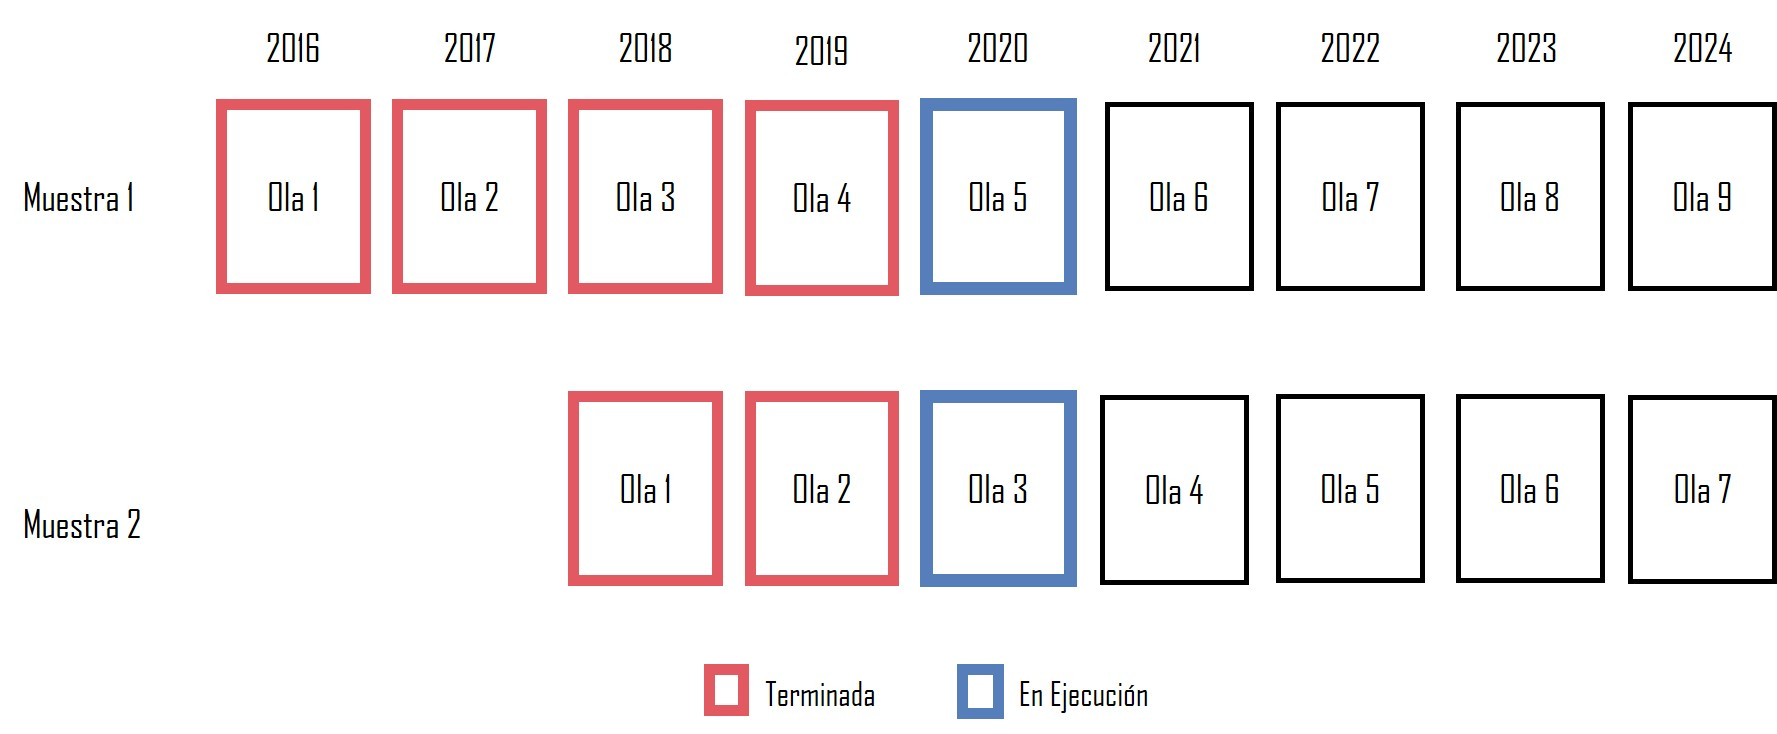
\includegraphics[width=1.5\linewidth,height=1.5\textheight]{inputs/images/longitudinal} \end{center}

\begin{itemize}
\item
  Unidad de Análisis: Individuos.
\item
  Población Objetivo: Hombres y mujeres de 18 a 75 años, residentes habituales de viviendas particulares ocupadas en zonas urbanas, localizadas en 40 ciudades (92 comunas, 13 regiones) del país.
\item
  Marco Muestral: Marco de muestreo de manzanas del pre-censo 2011, trabajo elaborado por el Centro de Inteligencia Territorial (CIT) de la Universidad Adolfo Ibáñez.
\item
  Diseño Muestral: Probabilístico, estratificado (por tamaño de ciudades), por conglomerados y multietápico.
\item
  Unidades de Muestreo: Primero se eligen ciudades (UPM), luego manzanas (USM), y sub-bloques y viviendas (UTM). La unidad final de selección es la persona.
\end{itemize}

\hypertarget{dimensiuxf3n-territorial-del-diseuxf1o-muestral}{%
\section{Dimensión Territorial del Diseño Muestral}\label{dimensiuxf3n-territorial-del-diseuxf1o-muestral}}

\begin{longtable}[]{@{}llcc@{}}
\toprule
\begin{minipage}[b]{0.20\columnwidth}\raggedright
Estrato\strut
\end{minipage} & \begin{minipage}[b]{0.20\columnwidth}\raggedright
Definición\strut
\end{minipage} & \begin{minipage}[b]{0.25\columnwidth}\centering
N° de ciudades en marco muestral\strut
\end{minipage} & \begin{minipage}[b]{0.25\columnwidth}\centering
N° de ciuades seleccionadas\strut
\end{minipage}\tabularnewline
\midrule
\endhead
\begin{minipage}[t]{0.20\columnwidth}\raggedright
Áreas metropolitana de Santiago\strut
\end{minipage} & \begin{minipage}[t]{0.20\columnwidth}\raggedright
\strut
\end{minipage} & \begin{minipage}[t]{0.25\columnwidth}\centering
1\strut
\end{minipage} & \begin{minipage}[t]{0.25\columnwidth}\centering
1\strut
\end{minipage}\tabularnewline
\begin{minipage}[t]{0.20\columnwidth}\raggedright
Áreas metropolitana de Valparaíso\strut
\end{minipage} & \begin{minipage}[t]{0.20\columnwidth}\raggedright
\strut
\end{minipage} & \begin{minipage}[t]{0.25\columnwidth}\centering
1\strut
\end{minipage} & \begin{minipage}[t]{0.25\columnwidth}\centering
1\strut
\end{minipage}\tabularnewline
\begin{minipage}[t]{0.20\columnwidth}\raggedright
Áreas metropolitana de Concepción\strut
\end{minipage} & \begin{minipage}[t]{0.20\columnwidth}\raggedright
\strut
\end{minipage} & \begin{minipage}[t]{0.25\columnwidth}\centering
1\strut
\end{minipage} & \begin{minipage}[t]{0.25\columnwidth}\centering
1\strut
\end{minipage}\tabularnewline
\begin{minipage}[t]{0.20\columnwidth}\raggedright
Ciudades grandes\strut
\end{minipage} & \begin{minipage}[t]{0.20\columnwidth}\raggedright
Más de 100.000 habitantes\strut
\end{minipage} & \begin{minipage}[t]{0.25\columnwidth}\centering
18\strut
\end{minipage} & \begin{minipage}[t]{0.25\columnwidth}\centering
8\strut
\end{minipage}\tabularnewline
\begin{minipage}[t]{0.20\columnwidth}\raggedright
Ciudades medianas\strut
\end{minipage} & \begin{minipage}[t]{0.20\columnwidth}\raggedright
Más de 30.000 habitantes\strut
\end{minipage} & \begin{minipage}[t]{0.25\columnwidth}\centering
28\strut
\end{minipage} & \begin{minipage}[t]{0.25\columnwidth}\centering
10\strut
\end{minipage}\tabularnewline
\begin{minipage}[t]{0.20\columnwidth}\raggedright
Ciudades pequeñas\strut
\end{minipage} & \begin{minipage}[t]{0.20\columnwidth}\raggedright
Más de 10.000 habitantes\strut
\end{minipage} & \begin{minipage}[t]{0.25\columnwidth}\centering
73\strut
\end{minipage} & \begin{minipage}[t]{0.25\columnwidth}\centering
19\strut
\end{minipage}\tabularnewline
\begin{minipage}[t]{0.20\columnwidth}\raggedright
Total\strut
\end{minipage} & \begin{minipage}[t]{0.20\columnwidth}\raggedright
\strut
\end{minipage} & \begin{minipage}[t]{0.25\columnwidth}\centering
122\strut
\end{minipage} & \begin{minipage}[t]{0.25\columnwidth}\centering
40\strut
\end{minipage}\tabularnewline
\bottomrule
\end{longtable}

\hypertarget{etapas-de-selecciuxf3n-en-el-diseuxf1o-muestral}{%
\chapter{Etapas de Selección en el Diseño Muestral}\label{etapas-de-selecciuxf3n-en-el-diseuxf1o-muestral}}

\begin{center}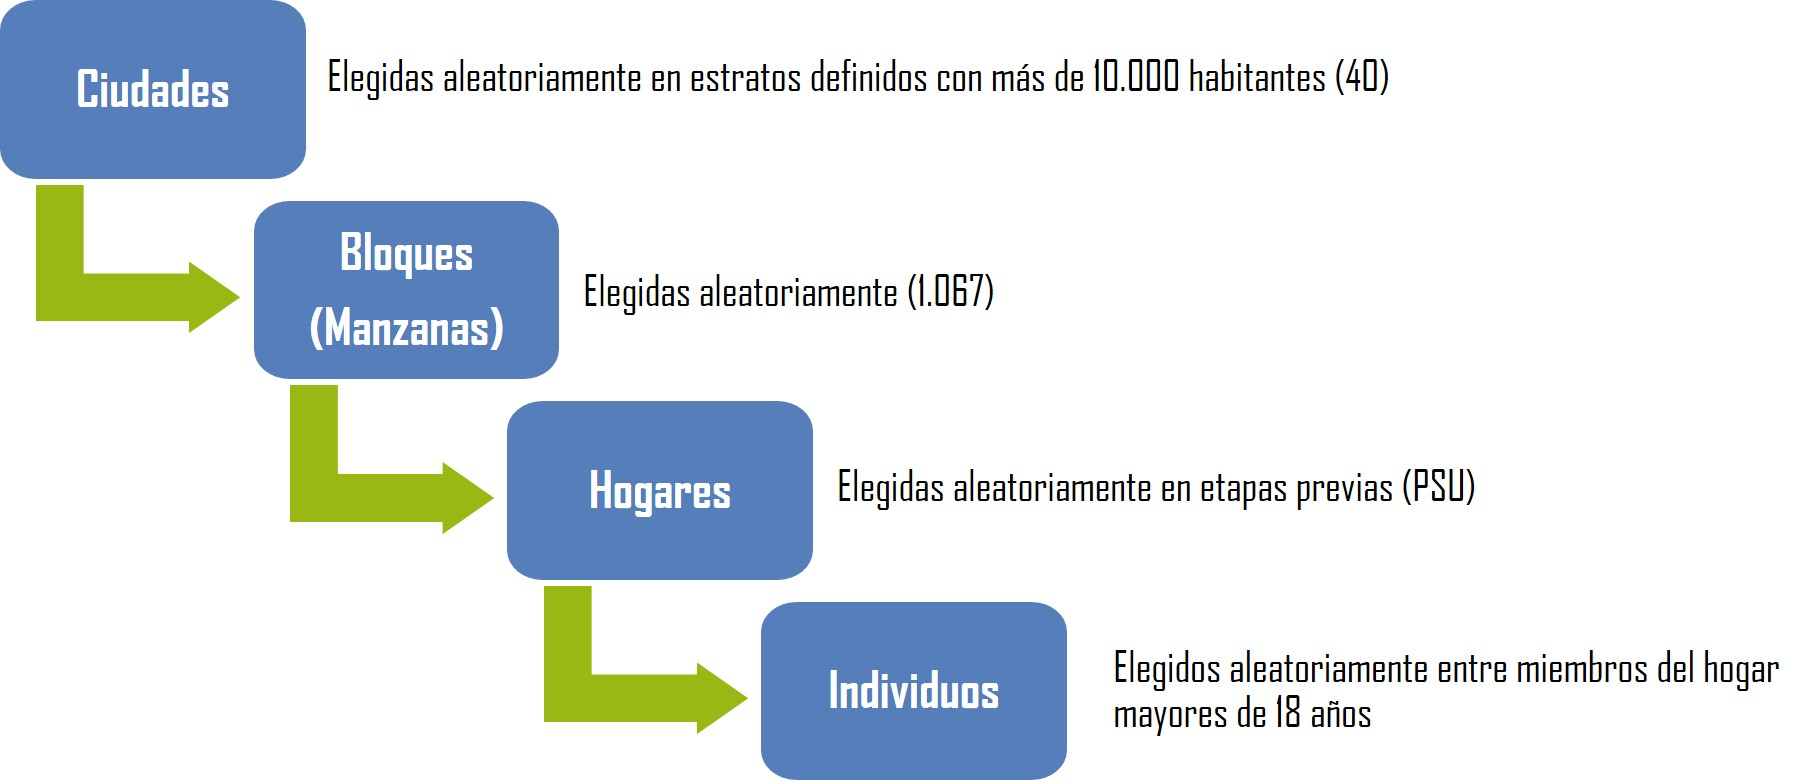
\includegraphics[width=1.5\linewidth,height=1.5\textheight]{inputs/images/etapas_seleccion} \end{center}

\textbf{Organismo Ejecutor}: Consultora Stephanie Eckman y Centro de Inteligencia Territorial (CIT) de la Universidad Adolfo Ibáñez (diseño muestral). Centro Micro Datos (CMD) de la Universidad de Chile (levantamiento, procesamiento de la información y construcción de factores de expansión).

\textbf{Entrenamiento y Ejecución}: Contratación de entrevistadores con experiencia en encuestas complejas y/o longitudinales. Capacitación centralizada y presencial para coordinadores de campo y un subconjunto de entrevistadores en Santiago (incluidos ejercicios prácticos para la implementación del cuestionario, uso de tabletas y protocolo de contacto). Actividades adicionales en otras regiones de Chile. Diseño de un Manual de entrevistador especializado para el proyecto.

\textbf{Operaciones de Control y Supervisión}: Entrega de incentivos monetarios para el encuestado (\$ 6.000 CLP) y de material sobre el estudio (ELSOC y COES). Acciones de seguimiento basadas en la información de contacto (correo electrónico para cumpleaños y días festivos). Los coordinadores de campo supervisan el trabajo de los entrevistadores, verificando el número de visitas, el contacto, la identidad del participante y algunas preguntas claves. El Centro Micro Datos realiza una supervisión interna de al menos el 10\% de la muestra (entrevistando nuevamente a algunos encuestados), verificando la duración y la respuesta de los participantes.

\hypertarget{descripciuxf3n-de-atriciuxf3n}{%
\chapter{Descripción de atrición}\label{descripciuxf3n-de-atriciuxf3n}}

\hypertarget{tamauxf1o-muestral}{%
\section{Tamaño muestral}\label{tamauxf1o-muestral}}

El diseño de ELSOC contempló entrevistar a 3.000 personas en su primera medición, reconociendo que año tras año, se reduciría el número de participantes, dado que algunos optarían voluntariamente por dejar de participar en el estudio y otras personas no podrían ser recontactadas o incluso algunas fallecerían. Este fenómeno es conocido como atrición, y pueden tener efectos nocivos sobre la utilidad de los datos longitudinales. Para cada año se planifica obtener un número de entrevistados (Muestra Objetivo) considerando una proyección de la atrición definida al momento de diseñar el estudio. ELSOC tiene buenos números en este aspecto. Incluso, en 2018 se logró recontactar a un número de participantes mayor al proyectado.

\begin{longtable}[]{@{}cccc@{}}
\toprule
Medición & Muestra Objetivo & Muestra Lograda & Porcentaje de Logro\tabularnewline
\midrule
\endhead
Muestra Original 2016 & 3000 & 2927 & 97.6\%\tabularnewline
Muestra Original 2017 & 2536 & 2473 & 97.5\%\tabularnewline
Muestra Original 2018 & 2131 & 2229 & 104.6\%\tabularnewline
Muestra Original 2019 & 1790 & 2153 & 120.3\%\tabularnewline
Muestra Refresco 2018 & 1500 & 1519 & 101.3\%\tabularnewline
Muestra Refresco 2019 & 1275 & 1264 & 99.1\%\tabularnewline
\bottomrule
\end{longtable}

\hypertarget{atriciuxf3n-de-la-muestra-original-y-muestra-refresco}{%
\section{Atrición de la Muestra Original y Muestra Refresco}\label{atriciuxf3n-de-la-muestra-original-y-muestra-refresco}}

\begin{longtable}[]{@{}cccc@{}}
\toprule
Medición & Muestra Lograda & Porcentaje Recuperado & Atrición\tabularnewline
\midrule
\endhead
Muestra Original 2016 & 2927 & - &\tabularnewline
Muestra Original 2017 & 2473 & 84.5\% & 15.5\%\tabularnewline
Muestra Original 2018 & 2229 & 90.1\% & 9.9\%\tabularnewline
Muestra Original 2019 & 2153 & 96.6\% & 3.4\%\tabularnewline
Muestra Refresco 2018 & 1519 & - &\tabularnewline
Muestra Refresco 2019 & 1264 & 83.2\% & 16.8\%\tabularnewline
\bottomrule
\end{longtable}

\hypertarget{atriciuxf3n-de-la-muestra-original-seguxfan-territorio}{%
\section{Atrición de la Muestra Original según Territorio}\label{atriciuxf3n-de-la-muestra-original-seguxfan-territorio}}

\begin{center}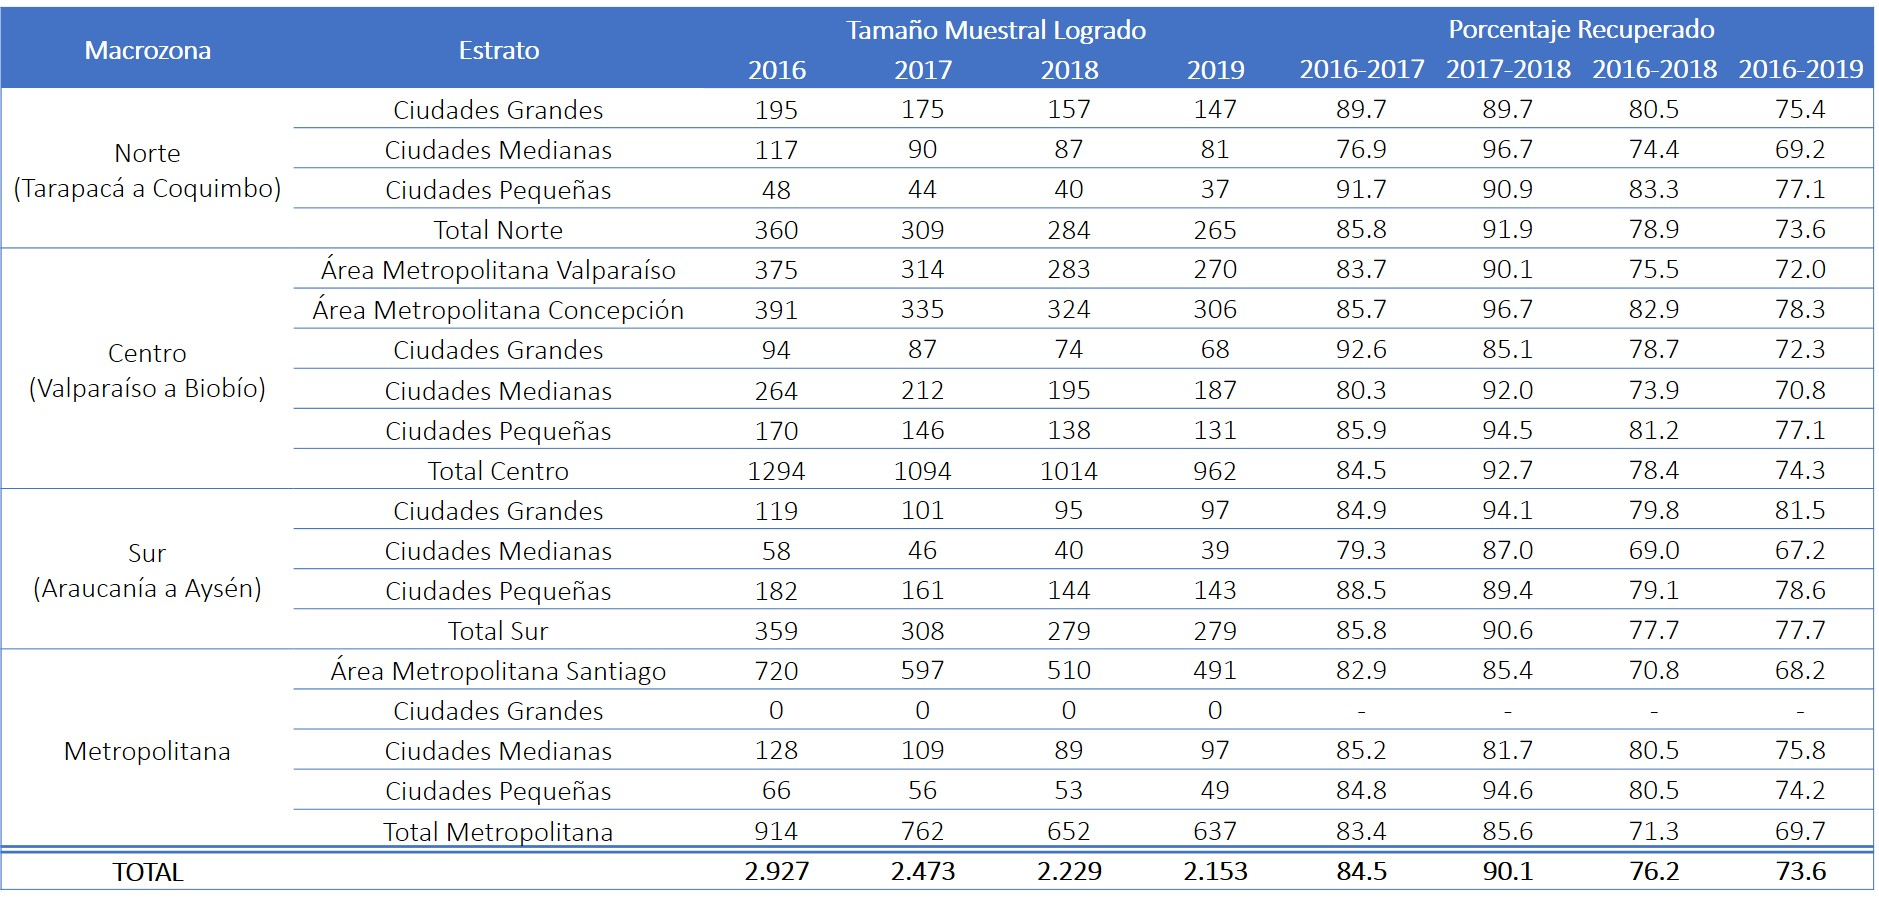
\includegraphics[width=1.5\linewidth,height=1.5\textheight]{inputs/images/atricion_territorio} \end{center}

\hypertarget{atriciuxf3n-muestral-original-seguxfan-sexo-y-edad}{%
\section{Atrición Muestral Original según sexo y edad*}\label{atriciuxf3n-muestral-original-seguxfan-sexo-y-edad}}

\begin{center}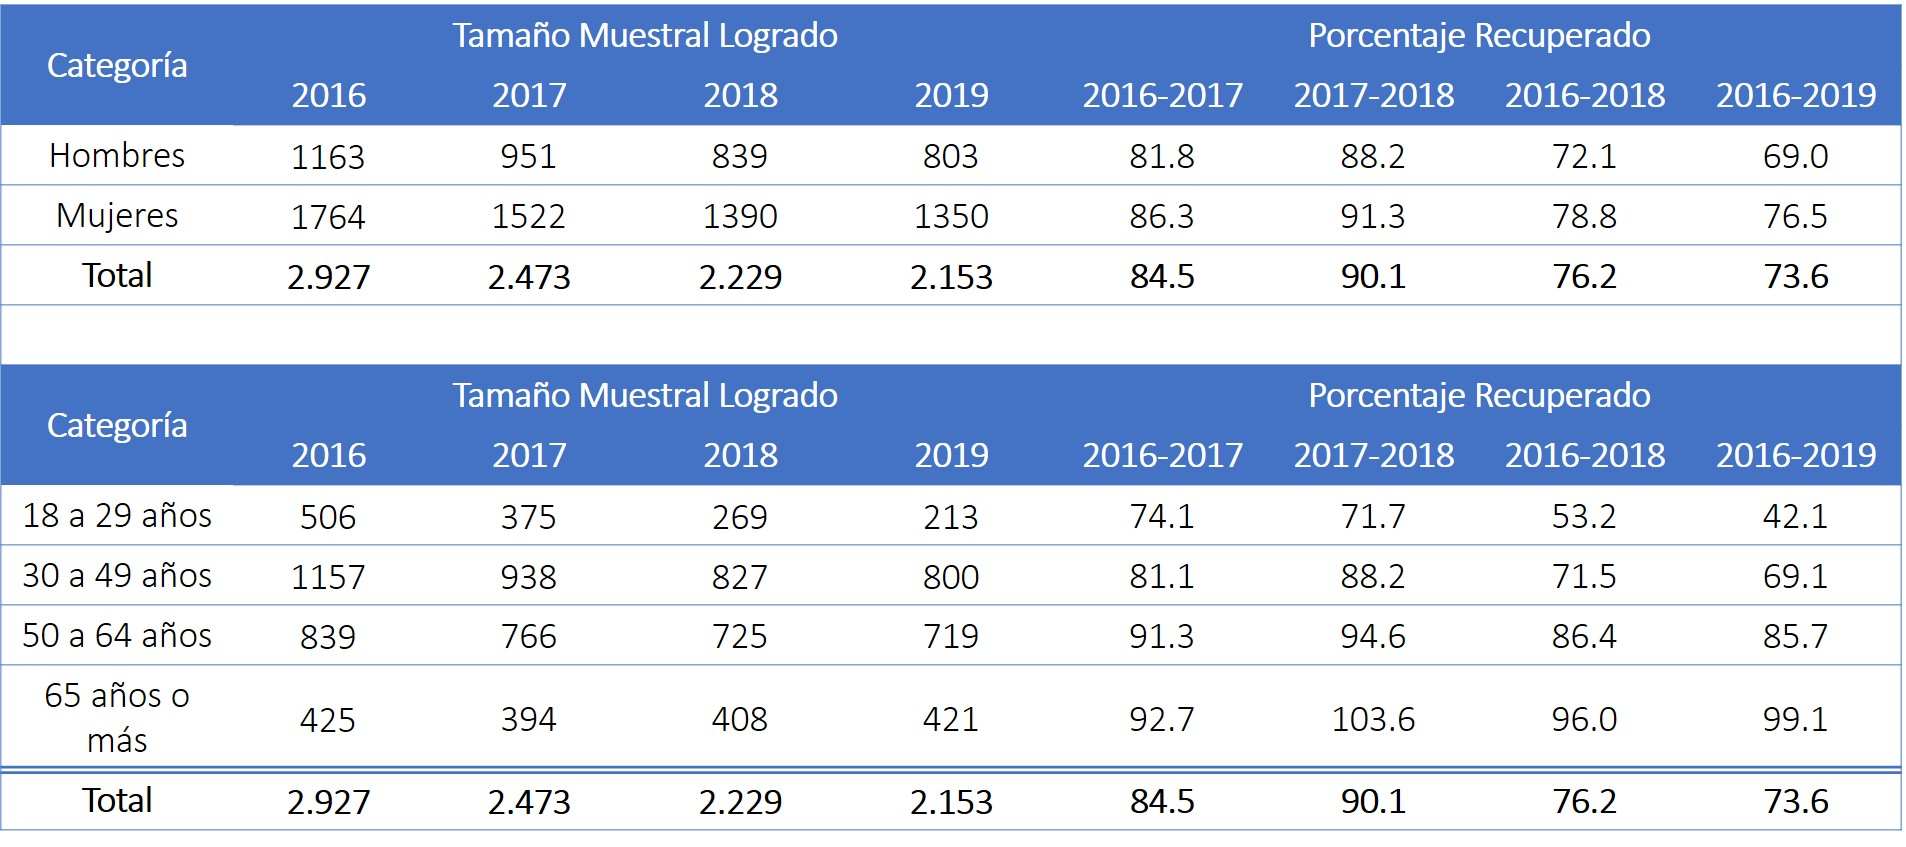
\includegraphics[width=1.5\linewidth,height=1.5\textheight]{inputs/images/atricion_sexo_edad} \end{center}

*El paso de los años entre olas hace que los sujetos cambien de categoría etaria. El porcentaje recuperado asociado a edad debe considerarse como indicativo.

\hypertarget{atriciuxf3n-de-la-muestra-refresco-seguxfan-territorio}{%
\section{Atrición de la Muestra refresco según Territorio}\label{atriciuxf3n-de-la-muestra-refresco-seguxfan-territorio}}

\begin{center}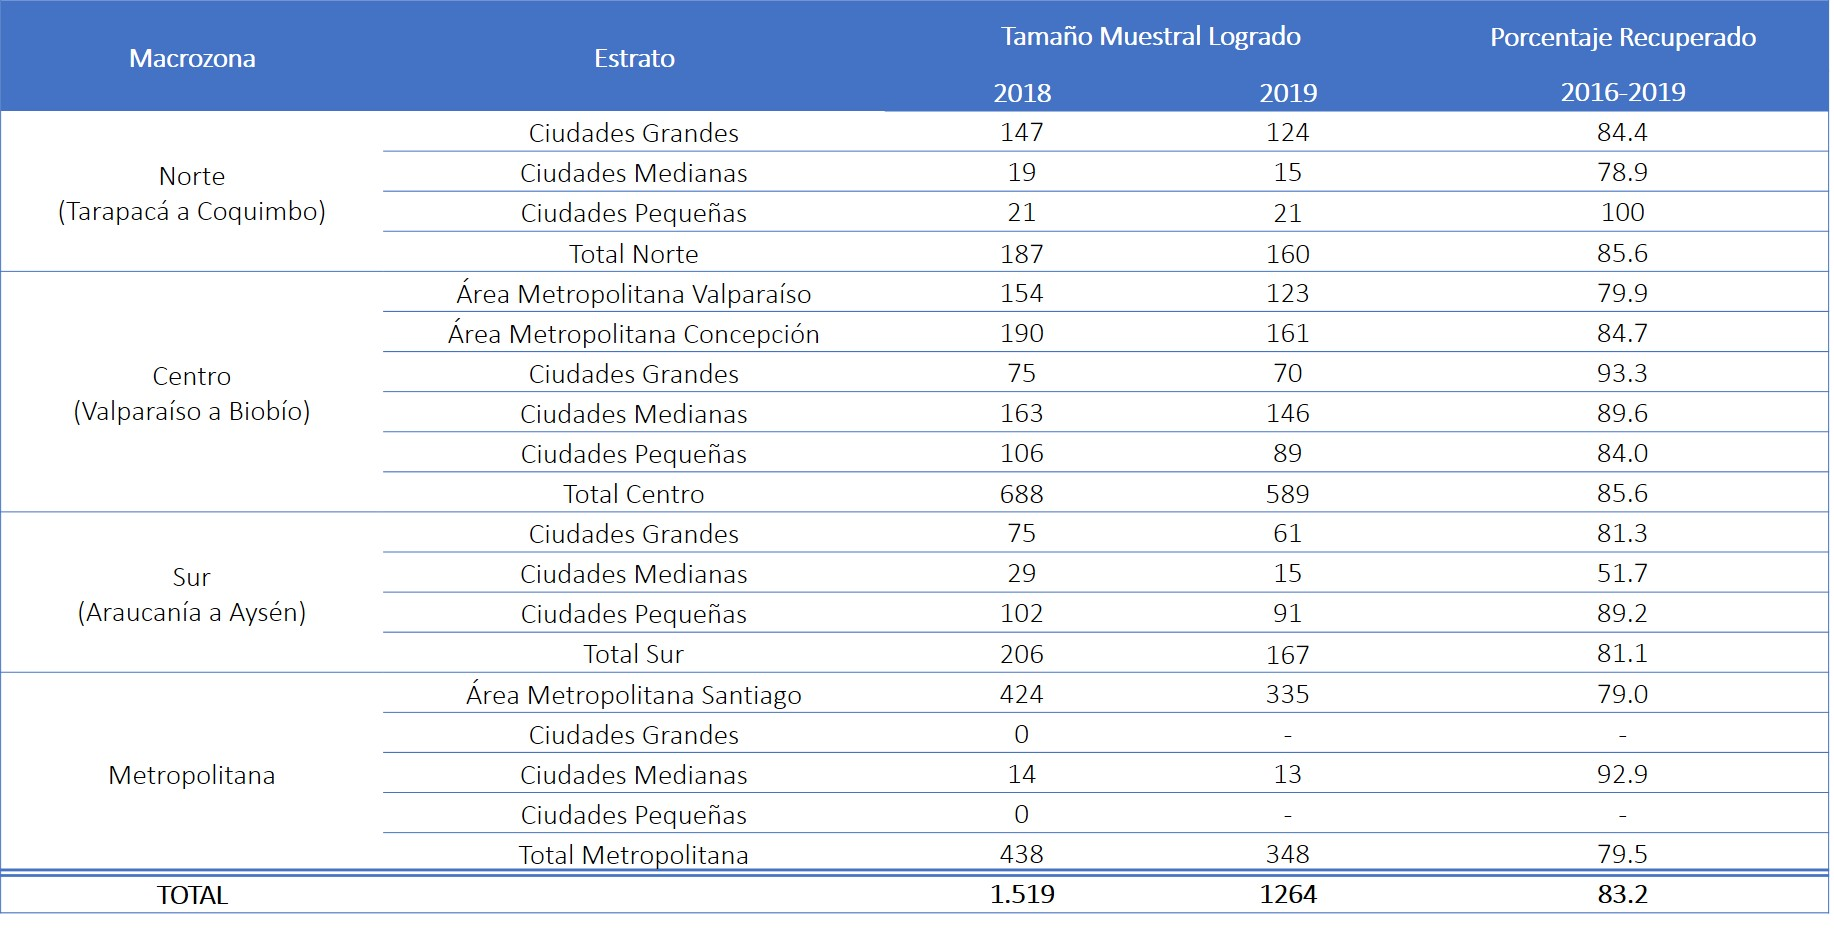
\includegraphics[width=1.5\linewidth,height=1.5\textheight]{inputs/images/atricion_ref_territorio} \end{center}

\hypertarget{atriciuxf3n-de-la-muestra-refresco-seguxfan-sexo-y-edad}{%
\section{Atrición de la Muestra Refresco según sexo y edad*}\label{atriciuxf3n-de-la-muestra-refresco-seguxfan-sexo-y-edad}}

\begin{center}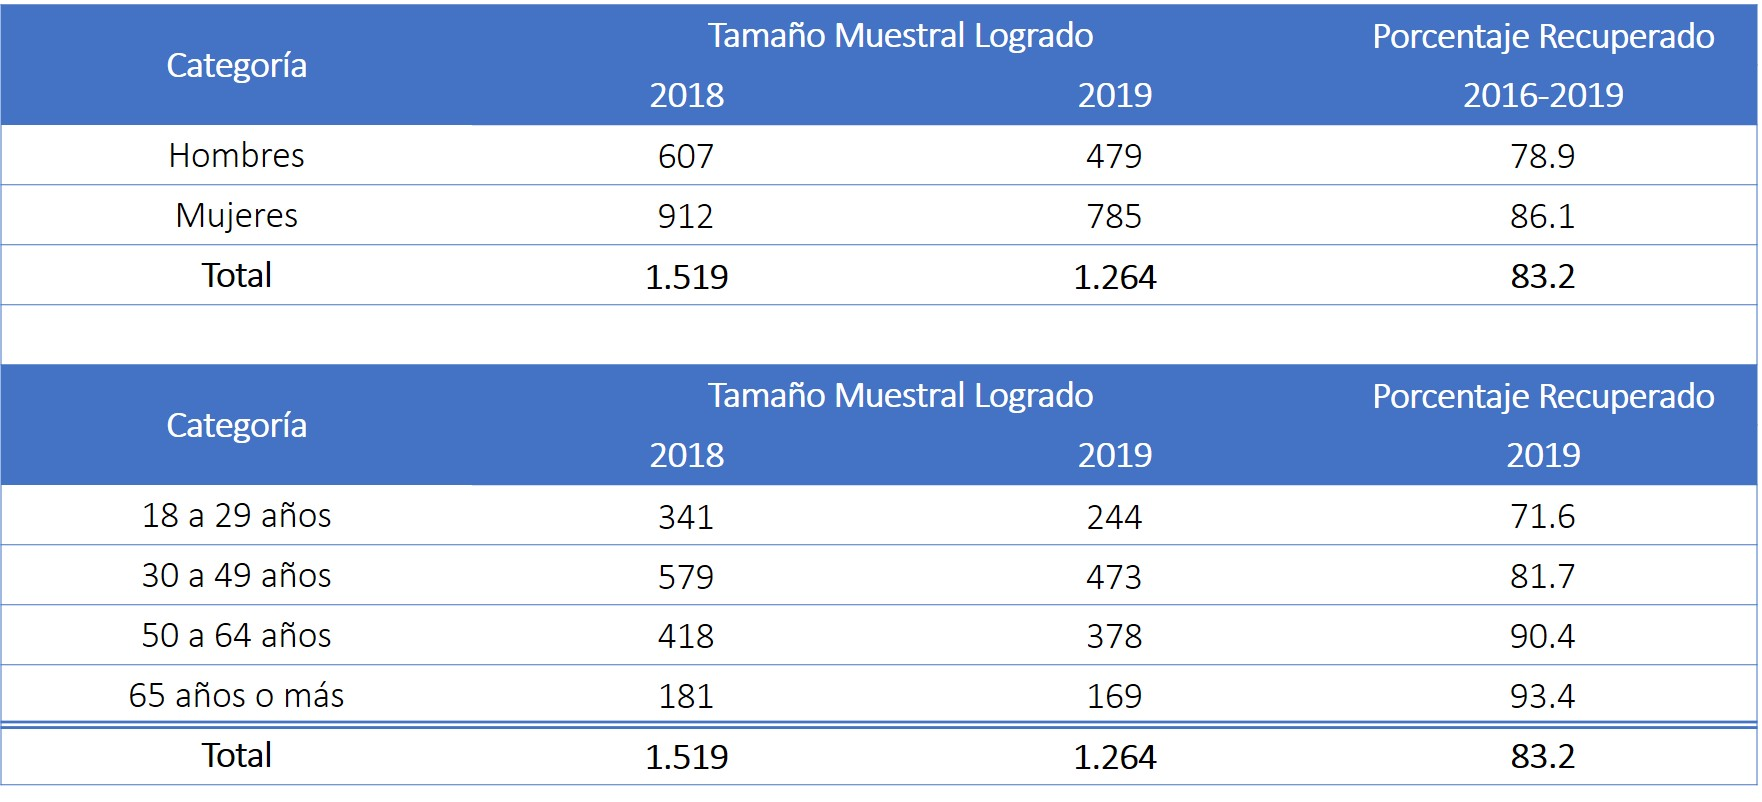
\includegraphics[width=1\linewidth,height=1\textheight]{inputs/images/atricion_ref_sexo_edad} \end{center}

*El paso de los años entre olas hace que los sujetos cambien de categoría etaria. El porcentaje recuperado asociado a edad debe considerarse como indicativo.

\hypertarget{composiciuxf3n-de-la-muestra}{%
\chapter{Composición de la Muestra}\label{composiciuxf3n-de-la-muestra}}

ELSOC ha ya completado cuatro mediciones anuales (2016, 2017, 2018 y 2019), lapso temporal dentro del cual es posible analizar la evolución de la sociedad chilena en todas las dimensiones medidas. Antes de proceder a la presentación de los principales hallazgos, este apartado caracteriza sociodemográficamente la muestra bajo estudio.

A continuación, describimos la muestra original de ELSOC en sus mediciones 2016 (N = 2.927), 2017 (N = 2.473), 2018 (N = 2.229) y 2019 (N = 2.153), según sexo, edad, educación, religión y zona de residencia. Todos los resultados presentados incorporan las principales características del diseño muestral complejo del estudio. Es decir, Se utiliza el ponderador muestral ajustado a población regional y sexo, estrato y conglomerado muestral.

\hypertarget{composiciuxf3n-de-muestra-seguxfan-sexo-y-ola-del-estudio}{%
\section{Composición de Muestra según sexo y ola del estudio}\label{composiciuxf3n-de-muestra-seguxfan-sexo-y-ola-del-estudio}}

\begin{center}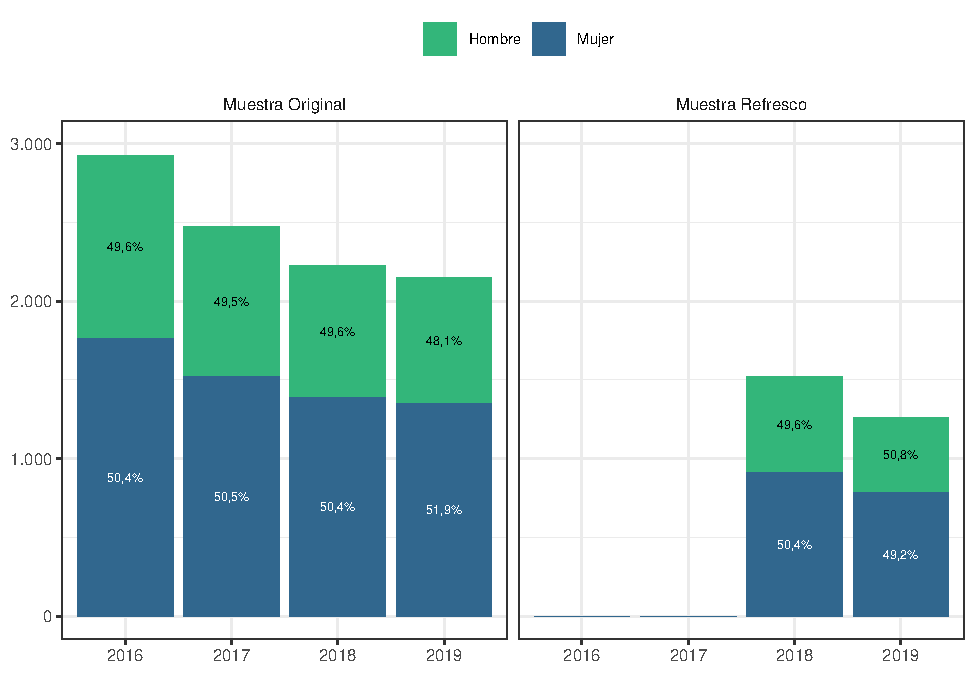
\includegraphics[width=0.75\linewidth]{concepto-medicion_files/figure-latex/unnamed-chunk-11-1} \end{center}

Nota: Resultados Ponderados (con Diseño Muestral Complejo)

\hypertarget{composiciuxf3n-de-muestra-seguxfan-edad-y-ola-del-estudio}{%
\section{Composición de Muestra según edad y ola del estudio}\label{composiciuxf3n-de-muestra-seguxfan-edad-y-ola-del-estudio}}

\begin{center}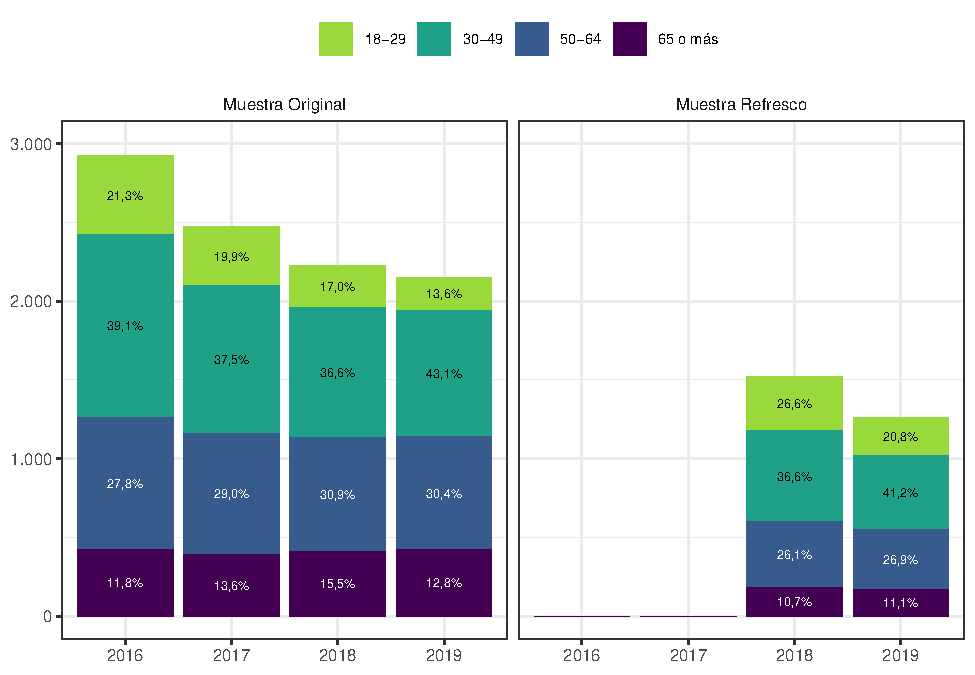
\includegraphics[width=0.75\linewidth]{concepto-medicion_files/figure-latex/unnamed-chunk-12-1} \end{center}

Nota: Resultados Ponderados (con Diseño Muestral Complejo)

\hypertarget{composiciuxf3n-de-muestra-seguxfan-educaciuxf3n-y-ola-del-estudio}{%
\section{Composición de Muestra según educación y ola del estudio}\label{composiciuxf3n-de-muestra-seguxfan-educaciuxf3n-y-ola-del-estudio}}

\begin{center}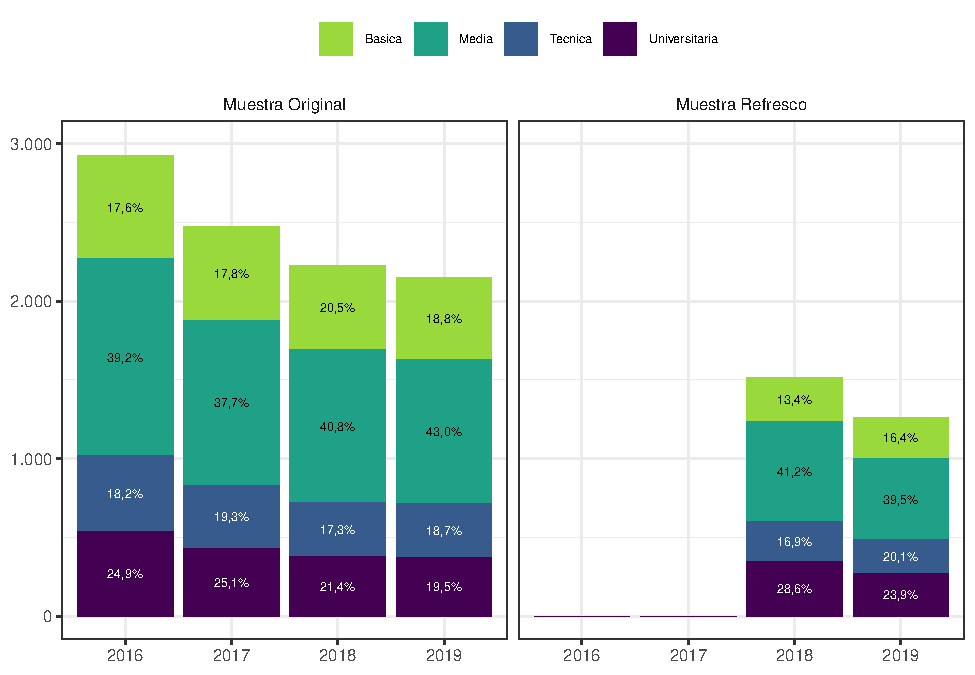
\includegraphics[width=0.75\linewidth]{concepto-medicion_files/figure-latex/unnamed-chunk-13-1} \end{center}

Nota: Resultados Ponderados (con Diseño Muestral Complejo)

\hypertarget{composiciuxf3n-de-muestra-seguxfan-religiuxf3n-y-ola-del-estudio}{%
\section{Composición de Muestra según religión y ola del estudio}\label{composiciuxf3n-de-muestra-seguxfan-religiuxf3n-y-ola-del-estudio}}

\begin{center}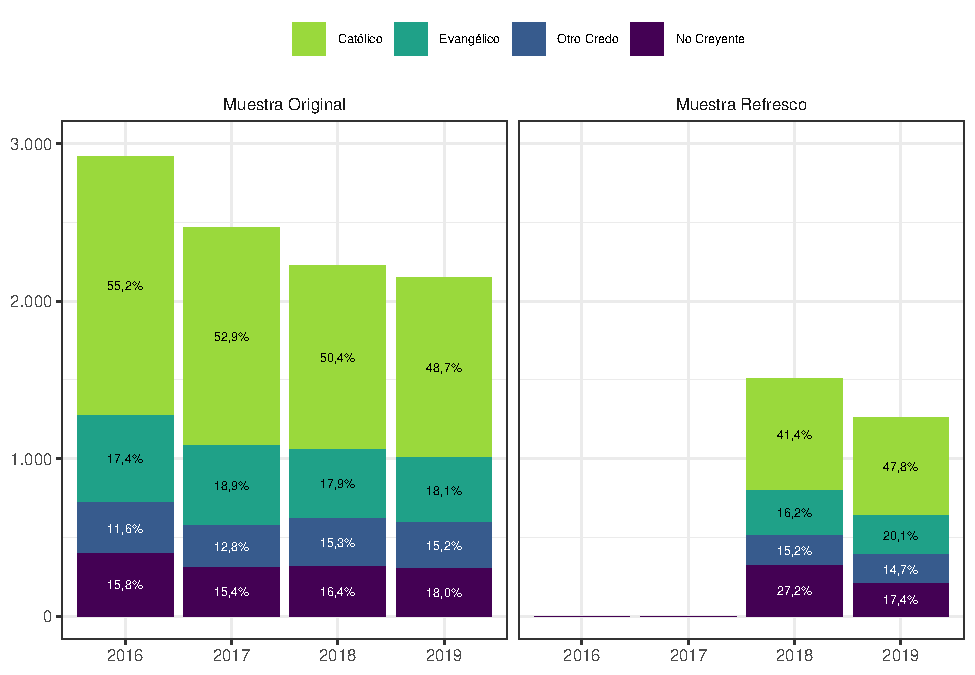
\includegraphics[width=0.75\linewidth]{concepto-medicion_files/figure-latex/unnamed-chunk-14-1} \end{center}

Nota: Resultados Ponderados (con Diseño Muestral Complejo)

\hypertarget{composiciuxf3n-de-muestra-seguxfan-zona-de-residencia-y-ola-del-estudio}{%
\section{Composición de Muestra según zona de residencia y ola del estudio}\label{composiciuxf3n-de-muestra-seguxfan-zona-de-residencia-y-ola-del-estudio}}

\begin{center}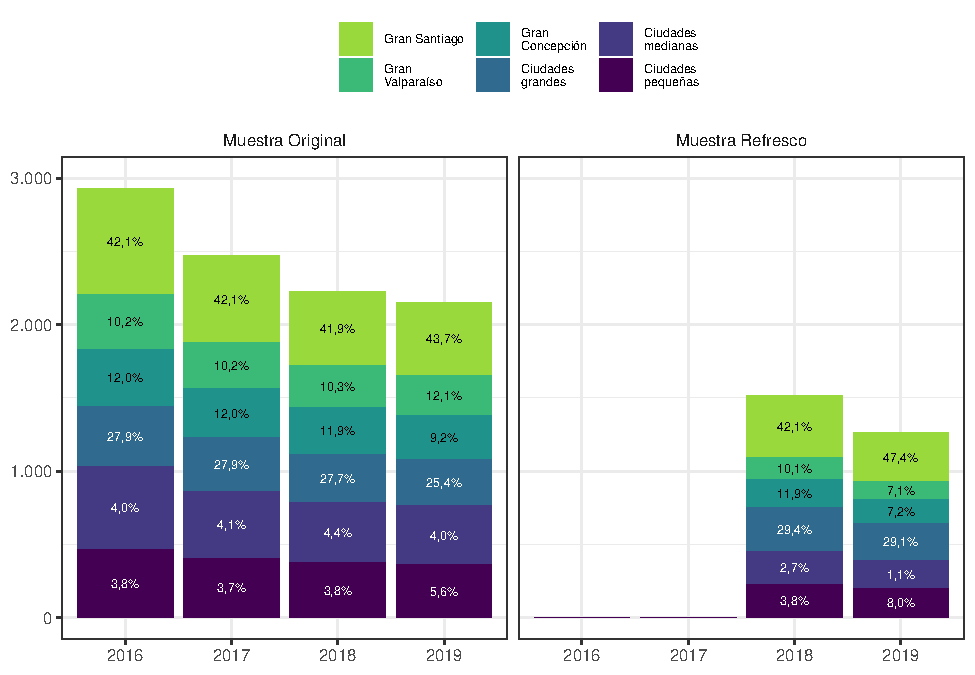
\includegraphics[width=0.75\linewidth]{concepto-medicion_files/figure-latex/unnamed-chunk-15-1} \end{center}

Nota: Resultados Ponderados (con Diseño Muestral Complejo)

\hypertarget{foco-en-el-cambio-individual}{%
\chapter{Foco en el cambio individual}\label{foco-en-el-cambio-individual}}

Radiografía del Cambio Social tiene como objetivo fundamental caracterizar la estabilidad y el cambio en opiniones, actitudes y conductas de los participantes a lo largo del tiempo, enfocándose en distintas dimensiones de la cohesión y conflicto en Chile.

Para el logro de dicho objetivo, el presente reporte se centrará en un subconjunto de participantes del estudio: los 2096 entrevistados que participaron en las cuatro primeras olas de ELSOC (como parte de la muestra original). Dicha submuestra será la base empírica de los hallazgos expuestos en las siguientes secciones.

A continuación se describe a este grupo de participantes según los mismos atributos sociodemográficos (sexo, edad, educación, zona de residencia y religión), considerando la primera medición. Todos los resultados presentados incorporan el diseño muestral complejo de la encuesta.

Nota 1: El promedio de edad de los participantes se ha incrementado entre estos años. También hay evidencia de un descenso en la identificación religiosa al comparar distintos años del estudio. Las otras variables no presentan variaciones relevantes a lo largo del tiempo.

Nota 2: Se utiliza el ponderador muestral ajustado a población regional y sexo, estrato y conglomerado muestral.

\hypertarget{distribuciuxf3n-de-sub-muestra-de-participantes-en-las-cuatro-olas-elsoc-seguxfan-sexo}{%
\section{Distribución de Sub-Muestra de Participantes en las cuatro olas ELSOC según sexo}\label{distribuciuxf3n-de-sub-muestra-de-participantes-en-las-cuatro-olas-elsoc-seguxfan-sexo}}

\begin{center}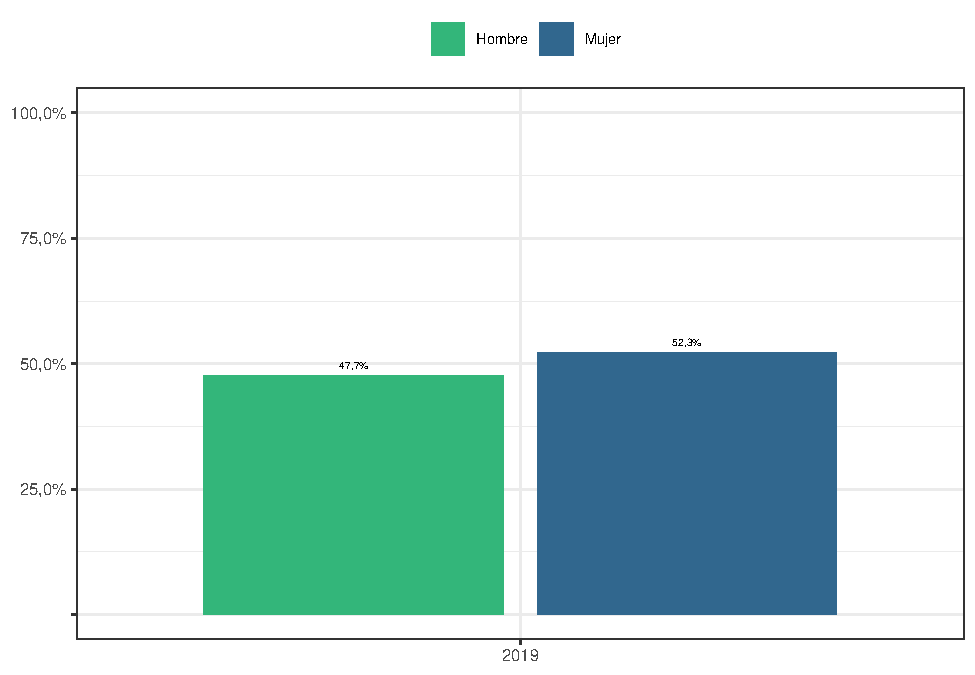
\includegraphics[width=0.75\linewidth]{concepto-medicion_files/figure-latex/unnamed-chunk-16-1} \end{center}

Nota: Resultados Ponderados (con Diseño Muestral Complejo)

\hypertarget{distribuciuxf3n-de-sub-muestra-de-participantes-en-las-cuatro-olas-elsoc-seguxfan-edad}{%
\section{Distribución de Sub-Muestra de Participantes en las cuatro olas ELSOC según edad}\label{distribuciuxf3n-de-sub-muestra-de-participantes-en-las-cuatro-olas-elsoc-seguxfan-edad}}

\begin{center}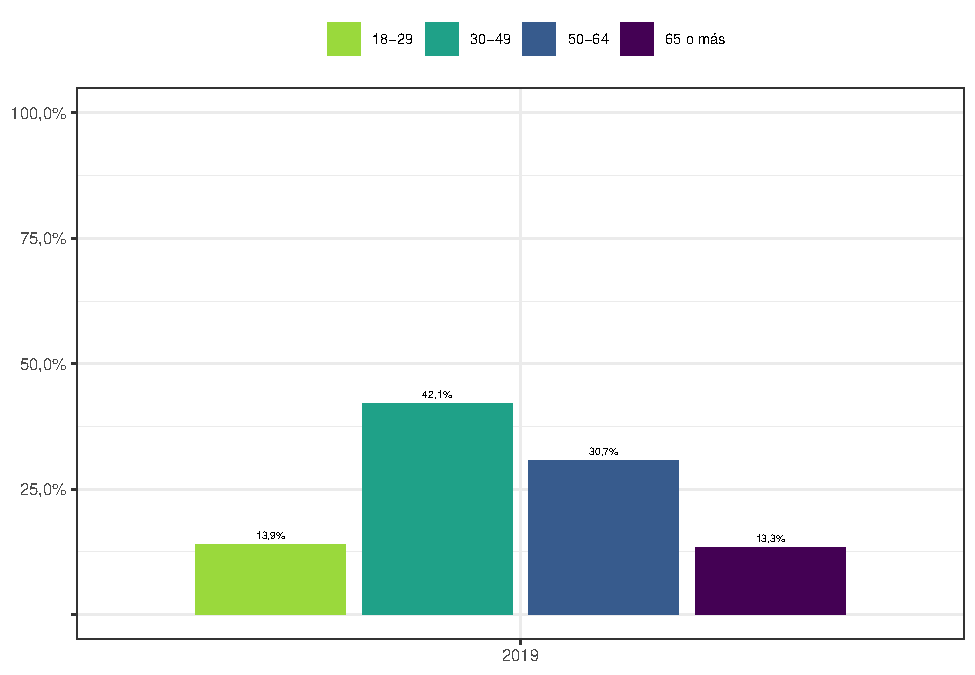
\includegraphics[width=0.75\linewidth]{concepto-medicion_files/figure-latex/unnamed-chunk-17-1} \end{center}

Nota: Resultados Ponderados (con Diseño Muestral Complejo)

\hypertarget{distribuciuxf3n-de-sub-muestra-de-participantes-en-las-cuatro-olas-elsoc-seguxfan-nivel-educacional}{%
\section{Distribución de Sub-muestra de Participantes en las cuatro olas ELSOC según Nivel educacional}\label{distribuciuxf3n-de-sub-muestra-de-participantes-en-las-cuatro-olas-elsoc-seguxfan-nivel-educacional}}

\begin{center}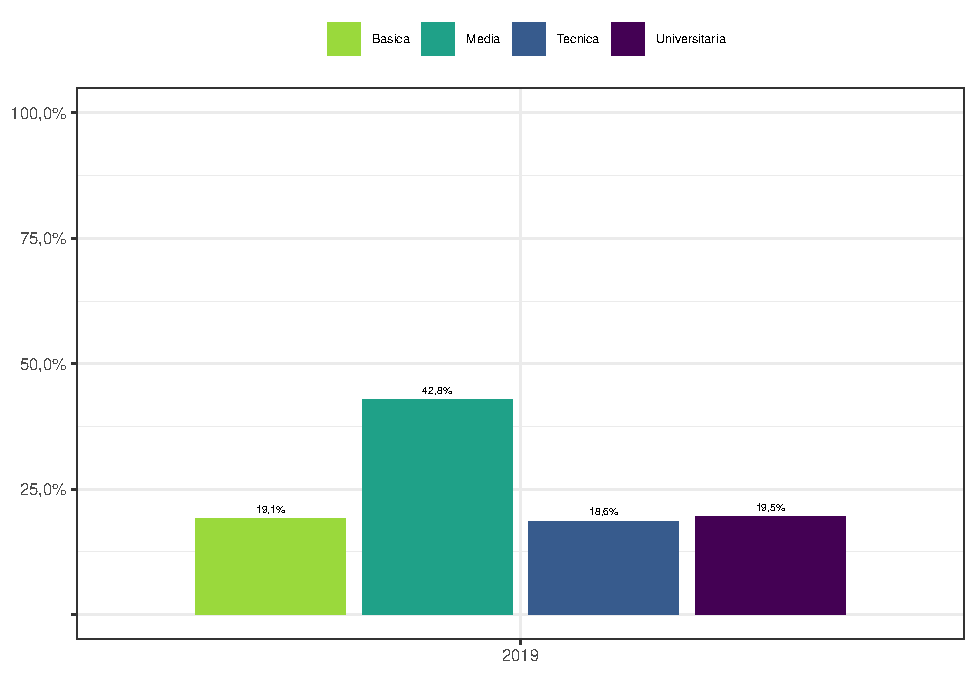
\includegraphics[width=0.75\linewidth]{concepto-medicion_files/figure-latex/unnamed-chunk-18-1} \end{center}

Nota: Resultados Ponderados (con Diseño Muestral Complejo)

\hypertarget{distribuciuxf3n-de-sub-muestra-de-participantes-en-las-cuatro-olas-elsoc-seguxfan-zona-de-residencia}{%
\section{Distribución de Sub-Muestra de Participantes en las cuatro olas ELSOC según zona de residencia}\label{distribuciuxf3n-de-sub-muestra-de-participantes-en-las-cuatro-olas-elsoc-seguxfan-zona-de-residencia}}

\begin{center}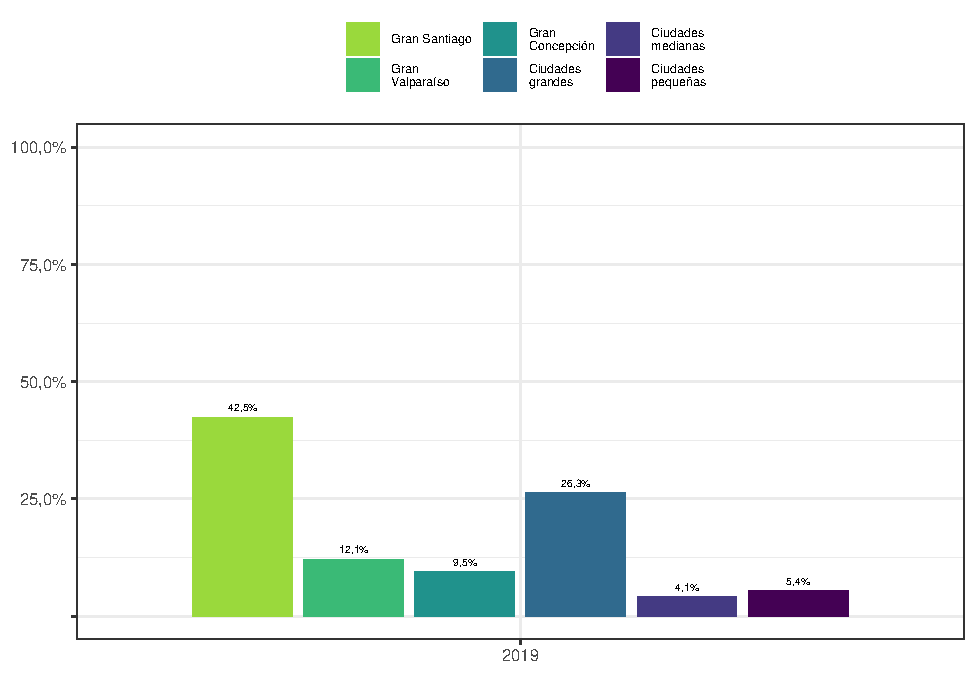
\includegraphics[width=0.75\linewidth]{concepto-medicion_files/figure-latex/unnamed-chunk-19-1} \end{center}

Nota: Resultados Ponderados (con Diseño Muestral Complejo)

  \bibliography{book.bib,packages.bib,book-ocs.bib}

\end{document}
